\documentclass[12pt]{article}

\usepackage{graphicx}
\graphicspath{{../Fichier_Image}}
\title{Hypothèse 3.(c) Porte Bureaux Regulation}
\author{Thibault Clodion}

\begin{document}

\maketitle % Permet d'afficher le titre, l'author etc

\underline{Hypothèse :} Certain bureaux (même grand) doivent avoir qu'une seule porte pour réguler les flux
\newline\newline
\underline{Expérience :}Des simulations avec le bâtiment en photo (le 7.), une où il a une porte (comme sur la photo) et une où il y en a deux dont une à gauche, donc il y aura plus de régulation des flux
\newline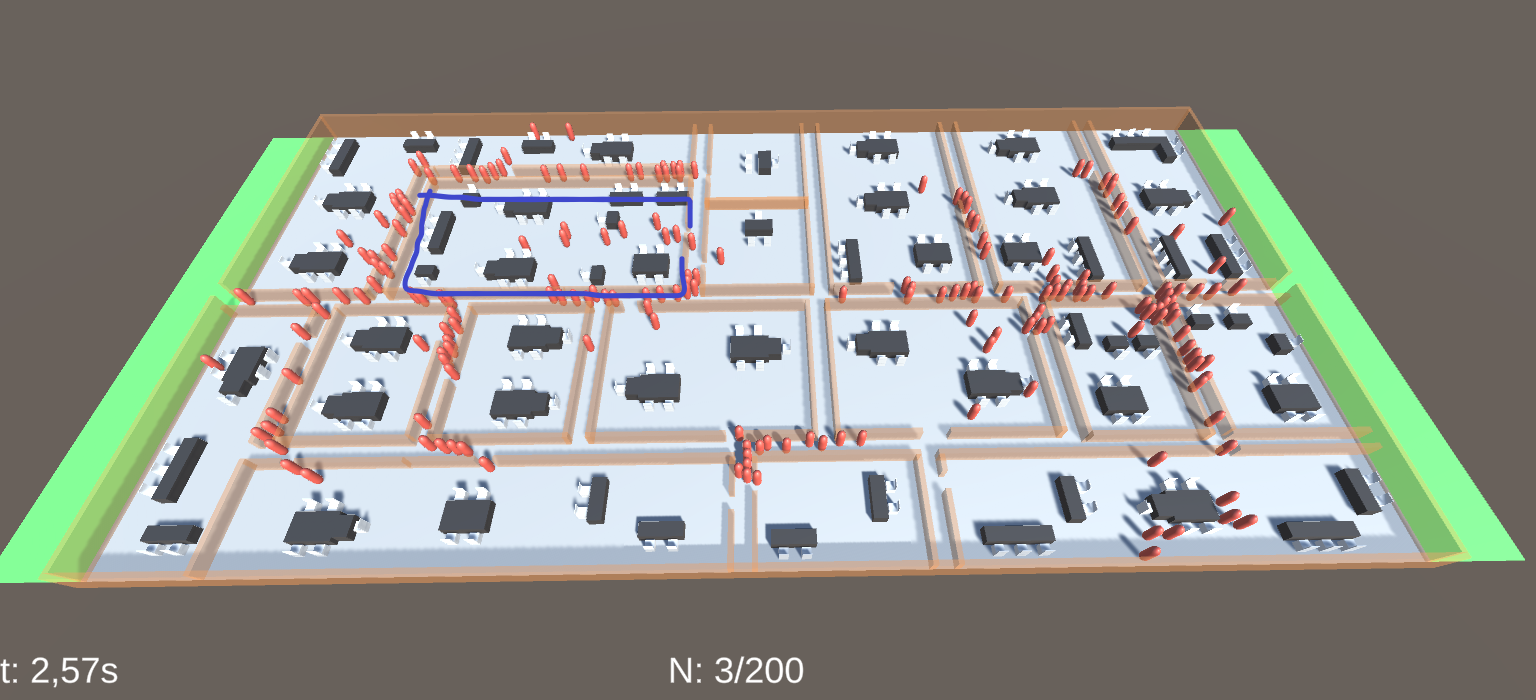
\includegraphics[scale=0.17]{7. bureau 1 porte.png}\newline
\newline
(peut-être le temps qu'ils fassent le tour revient à diviser le flux à voir.)
\newline\newline

Remarque : j'ai changé un peut le bâtiment 7 en modifiant les portes en bleu. Cela permet d'éviter des colisions qui biaiseraient les résultats (car le fait qu'il y est qu'une porte
aurait créer des collisions, c'est d'ailleurs un changement intéressant pour le 6.)
\newline
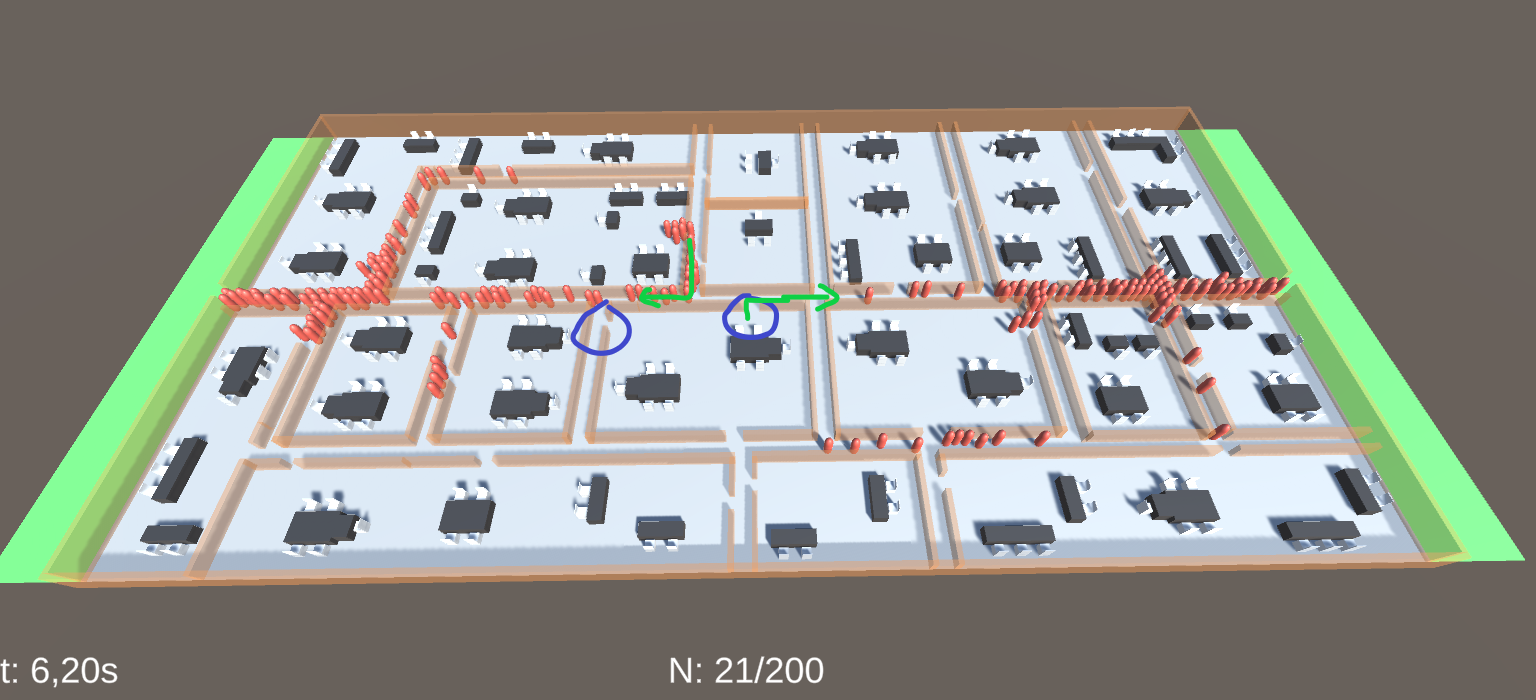
\includegraphics[scale=0.3]{3.(c) 7. avec 1 porte.png}
\newline\newline

3.(c) 7. avec 1 porte
\newline\newline
Temps moyen de dernière sortie : 23.10s
\newline
$\hspace*{0.2cm}$- Les personnes dans le bureaux ciblé rentrent dans le couloir par la droite et se retrouve donc peu en collision avec le reste du flux a gauche
(le phénomène se voit sur l'image au dessus)
\newline
$\hspace*{0.2cm}$- On a une régulation du flux qui permet d'éviter le nombre de collisions
\newline\newline

3.(c) 7. avec 2 portes
\newline\newline
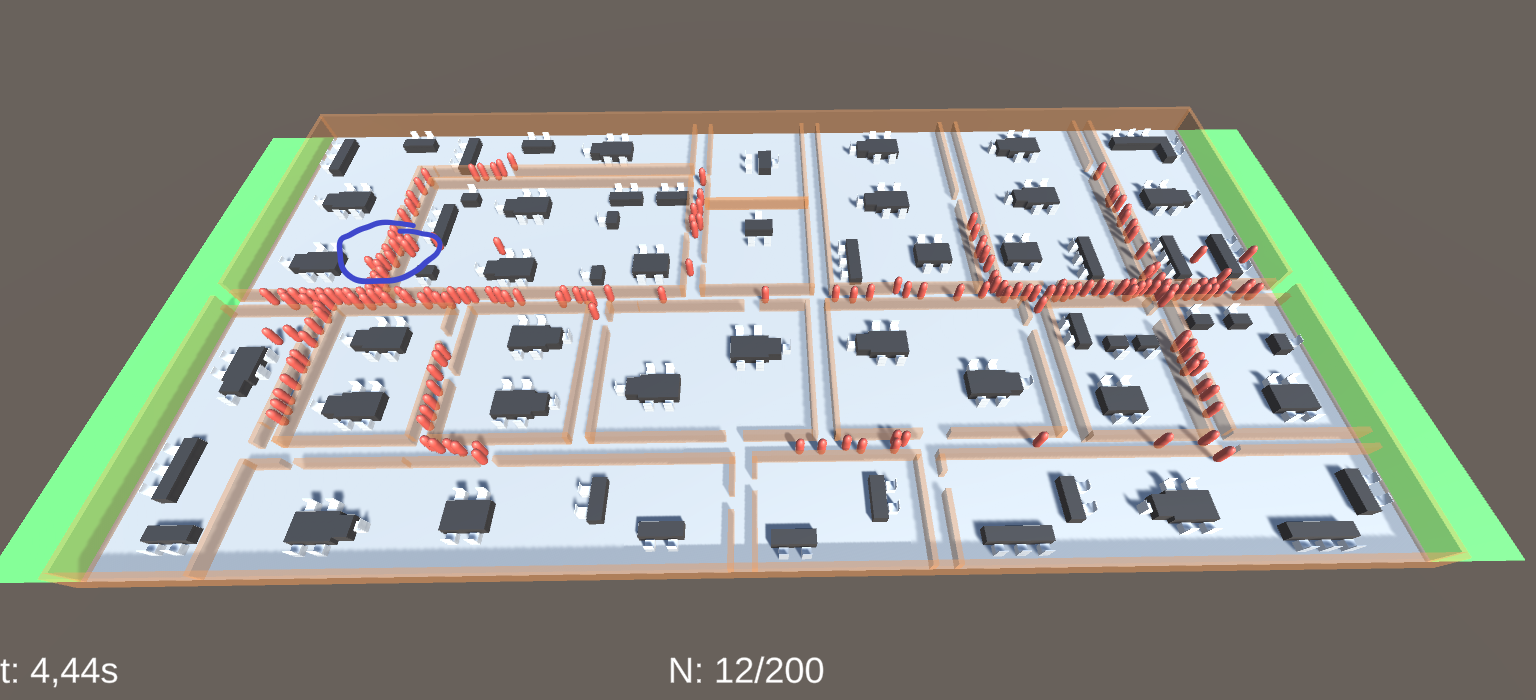
\includegraphics[scale=0.3]{3.(c) 7. avec 2 portes.png}
\newline\newline
Temps moyen de dernière sortie : 22.30s
\newline
$\hspace*{0.2cm}$- La porte ajouté, créer en effet plus de flux du côté gauche du bureau
\newline
$\hspace*{0.2cm}$- Il faut donc voir si l'importance du flux générer augmente en effet le temps
\newline\newline

\section{Résultat}

On remarque sur l'image avec 2 portes, qu'il reste un flux moyennement important qui vient de la droite du bureaux. De ce fait
les flux restent divisé et ce n'est pas vraiment ce que l'on voulait observer.
\newline\newline
Finalement lorsque le bureau a 2 portes, la sortie est plus rapide, ce qui n'est pas vraiment ce que je voulais observer.
\newline\newline
Je ne vais pas garder cette Hypothèse, je pense qu'il est finalement plus intéressant de voir comment placer les portes et eviter les croisements (6.).
\end{document}